% MICRO 2026 Survey Paper - ML Performance Models
% Using MICRO 59 ACM sigconf template
% Last compiled: 2026-02-07 (rebuild triggered)

%%
%% For submission and review of your manuscript please change the
%% command to \documentclass[manuscript, screen, review]{acmart}.
%%
\documentclass[sigconf, screen, review]{acmart}

%%
%% \BibTeX command to typeset BibTeX logo in the docs
\AtBeginDocument{%
  \providecommand\BibTeX{{%
    Bib\TeX}}}

%% Rights management information - for submission
\setcopyright{none}
\copyrightyear{2026}
\acmYear{2026}
\acmDOI{}

%% Conference information
\acmConference[MICRO 2026]{The 59th IEEE/ACM International Symposium on Microarchitecture}{November 2026}{Austin, TX, USA}
\acmISBN{}

%% Disable ACM reference format printing for submission
\settopmatter{printfolios=true}
\settopmatter{printacmref=false}

%% Anonymous submission
\author{Anonymous Author(s)}
\affiliation{%
  \institution{Under Review}
  \country{Anonymous}
}

%% Additional packages (acmart already loads amsmath, amsfonts, amssymb, booktabs)
\usepackage{multirow}
\usepackage{tikz}
\usetikzlibrary{shapes.geometric,arrows.meta,positioning,fit,backgrounds,patterns}
\usepackage{pgfplots}
\pgfplotsset{compat=1.18}
\usepgfplotslibrary{groupplots}
\usetikzlibrary{plotmarks}

% Custom commands
\newcommand{\todo}[1]{\textcolor{red}{[TODO: #1]}}

\begin{document}

\title{A Survey of High-Level Modeling and Simulation Methods for Modern Machine Learning Workloads}
\subtitle{\normalsize{MICRO 2026 Submission -- Confidential Draft -- Do NOT Distribute!!}}

%%
%% The abstract is a short summary of the work to be presented in the
%% article.

%%%%%% -- PAPER CONTENT STARTS-- %%%%%%%%

\begin{abstract}
As machine learning workloads grow in scale and complexity, architects need fast, accurate methods to predict performance across diverse hardware.
This survey analyzes 22 tools from 53 papers across architecture and systems venues (2016--2026), covering analytical models, trace-driven simulators, and ML-augmented hybrid techniques for DNN accelerators, GPUs, distributed training, and LLM inference serving.
We organize the literature by methodology type, target platform, and abstraction level, identifying a temporal validation lag where tools published before 2023 validated primarily on CNNs and finding that hybrid approaches achieve the best accuracy-speed trade-offs.
We conduct hands-on reproducibility evaluations of representative tools, assessing whether practitioners can reproduce each tool's functionality without the original authors' environment; tools with Docker-first deployment remain reproducible, while those relying on serialized ML models become unusable.
We identify open challenges including cross-workload generalization, kernel-to-end-to-end error composition, and emerging architecture support, providing practitioners tool selection guidance and researchers a roadmap for the field.
\end{abstract}

%%
%% Keywords
\keywords{ML workload performance prediction, DNN accelerator modeling, GPU simulation, distributed training simulation, LLM inference serving, design space exploration, survey}

\maketitle

% ==============================================================================
% INTRODUCTION
% ==============================================================================
\section{Introduction}
\label{sec:introduction}

Machine learning workloads have become the dominant consumers of compute across datacenters and edge devices.
Training and inference for CNNs, transformers, mixture-of-experts models, and LLMs demand hardware ranging from Google's TPU~\cite{tpuv1_2017,tpuv4_2023} to custom accelerators, creating a heterogeneous landscape where architects must predict performance before committing to costly hardware decisions.

The shift toward domain-specific architectures~\cite{hennessy2019golden} makes performance prediction both more important and more difficult.
Design space exploration, parallelization selection, and hardware-software co-design all require fast, accurate performance models---yet ML workloads pose unique challenges: diverse computational patterns (dense matrix operations, sparse accesses, communication-bound collectives) across GPUs, TPUs, custom accelerators, and multi-device clusters.

A rich ecosystem of modeling tools has emerged.
Analytical models (Timeloop~\cite{timeloop2019}, MAESTRO~\cite{maestro2019}) evaluate in microseconds with 5--15\% error.
Trace-driven simulators (ASTRA-sim~\cite{astrasim2023}, VIDUR~\cite{vidur2024}) replay execution traces for system-level modeling.
Hybrid approaches (NeuSight~\cite{neusight2025}) combine analytical structure with learned components to achieve 2.3\% error.
Yet no comprehensive survey organizes these methods for the practitioner who must select a tool for a specific task.
Existing surveys focus on ML \emph{techniques} for modeling~\cite{granite2022} or specific hardware~\cite{timeloop2019}; this survey fills that gap with a methodology-centric view that yields new architectural insights.

We make the following contributions:
\begin{itemize}
    \item A \textbf{methodology-centric taxonomy} organizing tools along three dimensions: methodology type, target platform, and abstraction level, with a coverage matrix identifying explicit research gaps (e.g., no trace-driven tools for accelerators, no hybrid tools for distributed systems).
    \item A \textbf{cross-methodology architectural analysis} revealing why structural decomposition aligned with hardware execution boundaries (loop nests for systolic arrays, tiles for GPU SMs, phases for serving) consistently outperforms methodology-agnostic approaches---an insight that cuts across subdomain boundaries and provides concrete design principles for future tools.
    \item \textbf{Hands-on reproducibility evaluation} of five representative tools, demonstrating that deployment methodology (Docker-first vs.\ serialized ML models) is a stronger predictor of usability than reported accuracy, with implications for tool design.
    \item An \textbf{error composition analysis} characterizing how kernel-level prediction errors propagate through the model-to-system abstraction stack, identifying the uncaptured inter-kernel overheads (launch latency, memory allocation, synchronization) that dominate the gap between kernel and end-to-end accuracy.
\end{itemize}

Figure~\ref{fig:timeline} illustrates the evolution of performance modeling tools from early analytical frameworks to modern hybrid approaches.

\begin{figure*}[t]
\centering
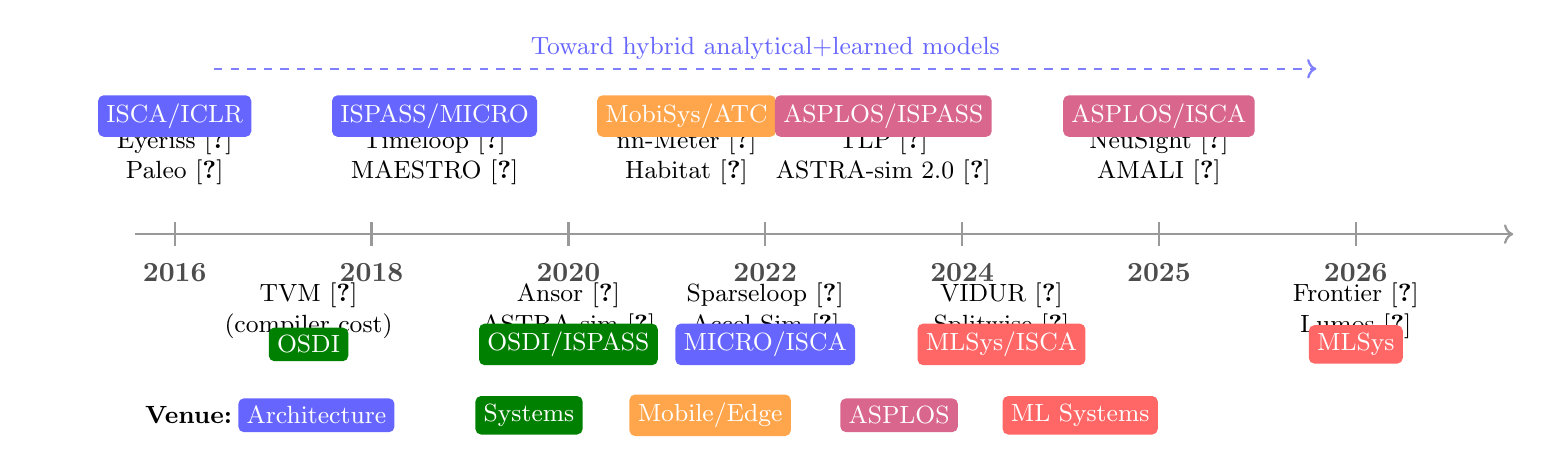
\begin{tikzpicture}[
    node distance=0.3cm,
    yearnode/.style={font=\normalsize\bfseries, text=black!70},
    eventnode/.style={font=\small, text width=3.5cm, align=center},
    catnode/.style={font=\small, text=white, rounded corners=2pt, inner sep=3pt}
]
% Timeline base
\draw[thick, ->, black!40] (0,0) -- (17.5,0);

% Year markers
\foreach \x/\year in {0.5/2016, 3/2018, 5.5/2020, 8/2022, 10.5/2024, 13/2025, 15.5/2026} {
    \draw[thick, black!40] (\x,-0.15) -- (\x,0.15);
    \node[yearnode, below] at (\x,-0.25) {\year};
}

% Events - staggered heights to avoid overlap
\node[eventnode, above] at (0.5,0.5) {Eyeriss~\cite{eyeriss2016}\\Paleo~\cite{paleo2017}};
\node[catnode, fill=blue!60] at (0.5,1.5) {ISCA/ICLR};

\node[eventnode, below] at (2.2,-0.5) {TVM~\cite{tvm2018}\\(compiler cost)};
\node[catnode, fill=green!50!black] at (2.2,-1.4) {OSDI};

\node[eventnode, above] at (3.8,0.5) {Timeloop~\cite{timeloop2019}\\MAESTRO~\cite{maestro2019}};
\node[catnode, fill=blue!60] at (3.8,1.5) {ISPASS/MICRO};

\node[eventnode, below] at (5.5,-0.5) {Ansor~\cite{ansor2020}\\ASTRA-sim~\cite{astrasim2020}};
\node[catnode, fill=green!50!black] at (5.5,-1.4) {OSDI/ISPASS};

\node[eventnode, above] at (7,0.5) {nn-Meter~\cite{nnmeter2021}\\Habitat~\cite{habitat2021}};
\node[catnode, fill=orange!70] at (7,1.5) {MobiSys/ATC};

\node[eventnode, below] at (8,-0.5) {Sparseloop~\cite{sparseloop2022}\\Accel-Sim~\cite{accelsim2020}};
\node[catnode, fill=blue!60] at (8,-1.4) {MICRO/ISCA};

\node[eventnode, above] at (9.5,0.5) {TLP~\cite{tlp2023}\\ASTRA-sim 2.0~\cite{astrasim2023}};
\node[catnode, fill=purple!60] at (9.5,1.5) {ASPLOS/ISPASS};

\node[eventnode, below] at (11,-0.5) {VIDUR~\cite{vidur2024}\\Splitwise~\cite{splitwise2024}};
\node[catnode, fill=red!60] at (11,-1.4) {MLSys/ISCA};

\node[eventnode, above] at (13,0.5) {NeuSight~\cite{neusight2025}\\AMALI~\cite{amali2025}};
\node[catnode, fill=purple!60] at (13,1.5) {ASPLOS/ISCA};

\node[eventnode, below] at (15.5,-0.5) {Frontier~\cite{frontier2025}\\Lumos~\cite{lumos2025}};
\node[catnode, fill=red!60] at (15.5,-1.4) {MLSys};

% Trend arrow
\draw[thick, ->, blue!50, dashed] (1,2.1) -- (15,2.1);
\node[font=\small, text=blue!60, above] at (8,2.1) {Toward hybrid analytical+learned models};

% Color legend
\node[font=\small\bfseries, anchor=west] at (0,-2.3) {Venue:};
\node[catnode, fill=blue!60] at (2.3,-2.3) {Architecture};
\node[catnode, fill=green!50!black] at (5,-2.3) {Systems};
\node[catnode, fill=orange!70] at (7.3,-2.3) {Mobile/Edge};
\node[catnode, fill=purple!60] at (9.7,-2.3) {ASPLOS};
\node[catnode, fill=red!60] at (12,-2.3) {ML Systems};

\end{tikzpicture}
\caption{Evolution of performance modeling tools for ML workloads (2016--2026). Colors indicate publication venue category. Early analytical frameworks (Eyeriss, Paleo) gave way to systematic accelerator modeling (Timeloop, MAESTRO) and distributed training simulation (ASTRA-sim). Recent work targets LLM-specific modeling (VIDUR, Frontier) and hybrid approaches (NeuSight).}
\label{fig:timeline}
\end{figure*}

% ==============================================================================
% SURVEY METHODOLOGY
% ==============================================================================
\section{Survey Methodology}
\label{sec:methodology}

We searched ACM Digital Library, IEEE Xplore, Semantic Scholar, and arXiv using terms related to ML performance modeling, with backward/forward citation tracking from seminal works.
Target venues include architecture (MICRO, ISCA, HPCA, ASPLOS), systems (MLSys, OSDI, SOSP, NSDI), and related (NeurIPS, MobiSys, DAC, ISPASS).
Papers must propose or evaluate a tool for predicting ML workload performance with quantitative evaluation; we exclude non-performance tasks and general-purpose workloads.
From 287 initial candidates, title/abstract screening yielded 118 papers; full-text review reduced the set to 53 that met all criteria, supplemented by 12 foundational works for context.
We cover 2016--2026 and classify each paper by \emph{methodology type} (analytical, simulation, trace-driven, ML-augmented, hybrid), \emph{target platform}, and \emph{abstraction level} (kernel, model, system).

\textbf{Related surveys and scope boundaries.}
Prior surveys address adjacent topics: Rakhshanfar and Zarandi~\cite{rakhshanfar2021survey} survey ML for processor DSE; Sze et al.~\cite{sze2017efficient} treat DNN hardware design (the foundation for Timeloop/MAESTRO); simulators such as GPGPU-Sim~\cite{gpgpusim2009}, gem5~\cite{binkert2011gem5}, and SST~\cite{sst2012} have been extensively used as validation targets in the performance modeling literature; and MLPerf~\cite{mlperf_training2020,mlperf_inference2020} standardizes \emph{measurement} rather than \emph{prediction}.
Early ML accelerator modeling (2014--2018) established foundational approaches: DianNao~\cite{diannao2014} introduced analytical dataflow modeling for dedicated accelerators, Eyeriss~\cite{eyeriss2016} systematized row-stationary dataflow analysis, and Paleo~\cite{paleo2017} pioneered layer-wise analytical estimation.
The closest prior work, Dudziak et al.~\cite{latencypredictorsnas2024}, compares edge device predictors for NAS; we broaden to the full landscape.

\textbf{Proprietary and vendor tools.}
NVIDIA's Nsight Compute~\cite{nsightcompute2019} and Nsight Systems are the most widely-used GPU profiling tools in practice; Google's internal TPU models underpin production scheduling but are undocumented.
We exclude these from evaluation as they cannot be independently reproduced, though surveyed tools frequently validate against Nsight Compute data.

\textbf{Compiler cost models and capacity planning.}
Beyond TVM/Ansor/TLP, relevant compiler models include Halide's autoscheduler~\cite{halide2013} (pioneered learned cost models), MLIR-based cost models~\cite{mlir2020}, and Triton's~\cite{triton2019} heuristic GPU kernel cost model.
At the system level, Pollux~\cite{pollux2021} and Sia~\cite{sia2023} use performance models for cluster scheduling and capacity planning---a distinct use case (optimizing workload placement) that shares modeling techniques with our surveyed tools.

This survey differs from all prior work by spanning the full methodology spectrum across all major platforms with reproducibility evaluation.

% ==============================================================================
% BACKGROUND
% ==============================================================================
\section{Background}
\label{sec:background}

\subsection{ML Workload Characteristics}
\label{subsec:workload-characteristics}

ML workloads are expressed as computation graphs whose operator shapes are statically known and amenable to analytical modeling. Frameworks such as PyTorch~\cite{pytorch2019} and TensorFlow~\cite{tensorflow2016} compile these graphs for execution, though MoE and dynamic inference introduce input-dependent control flow.
Performance depends on tensor-to-memory mapping (dataflow, tiling), KV cache management for LLM inference~\cite{vllm2023}, and at scale, compute--memory--network interactions across data, tensor, pipeline, and expert parallelism~\cite{llama3scaling2025}.
LLM inference splits into compute-bound prefill and memory-bound decode phases~\cite{splitwise2024}, both modeled under batched serving~\cite{sarathi2024,orca2022}.
Foundation model training introduces additional modeling challenges: long-context attention with quadratic memory scaling, activation checkpointing that trades compute for memory, and mixed-precision training where numerical format affects both speed and convergence~\cite{llama3scaling2025}.

\subsection{Modeling Methodologies}
\label{subsec:modeling-methodologies}

We classify approaches into five categories.
\textbf{Analytical models} express performance as closed-form functions (e.g., the roofline model~\cite{williams2009roofline}), offering microsecond evaluation but requiring per-architecture derivation.
\textbf{Cycle-accurate simulators} (GPGPU-Sim~\cite{gpgpusim2009}, Accel-Sim~\cite{accelsim2020}) achieve high fidelity at $1000$--$10000\times$ slowdown, serving primarily as validation oracles for the high-level methods that are the focus of this survey.
\textbf{Trace-driven simulators} (ASTRA-sim~\cite{astrasim2023}, VIDUR~\cite{vidur2024}) trade fidelity for orders-of-magnitude speedup.
\textbf{ML-augmented approaches} learn from profiling data (nn-Meter~\cite{nnmeter2021}) but may not generalize beyond training distributions.
\textbf{Hybrid approaches} combine analytical structure with learned components (NeuSight~\cite{neusight2025}, Habitat~\cite{habitat2021}), aiming to balance accuracy, speed, and interpretability.

\subsection{Metrics and Evaluation}
\label{subsec:problem-formulation}

Accuracy metrics---MAPE, RMSE, and rank correlation---vary across the literature, and differences in benchmarks, hardware targets, and evaluation protocols limit direct comparison (Section~\ref{sec:comparison}).
Ground-truth measurements rely on hardware performance counters (PAPI~\cite{papi2000}, LIKWID~\cite{likwid2010}) or vendor profilers (Nsight Compute~\cite{nsightcompute2019}).

% ==============================================================================
% TAXONOMY
% ==============================================================================
\section{Taxonomy}
\label{sec:taxonomy}

We organize the literature along three dimensions.
The \emph{primary axis} is methodology type---how a tool predicts performance---because methodology determines the fundamental trade-offs between accuracy, speed, interpretability, and data requirements.
The \emph{secondary axes} are target platform and abstraction level, which together determine the scope and applicability of each tool.
We additionally characterize tools by workload coverage, identifying a temporal validation lag: tools published during the CNN era naturally validated on CNN workloads, while post-2023 tools increasingly target transformers and LLMs.

Table~\ref{tab:taxonomy-matrix} provides a unified view combining the coverage matrix (number of surveyed tools per methodology--platform cell) with trade-off profiles, with empty cells highlighting research gaps.
The dominant pairings are: analytical models for accelerators, cycle-accurate simulation for GPUs/CPUs, trace-driven simulation for distributed systems, and ML-augmented approaches for edge devices.

% --- Unified Taxonomy Table (merged from Tables 1+2, issue #192) ---
\begin{table*}[t]
\centering
\caption{Methodology taxonomy: coverage matrix and trade-off profile.
Platform columns show the number of surveyed tools per cell; \textbf{0} indicates an explicit research gap.
Speed, data requirements, and interpretability determine practical applicability; the failure mode column identifies the primary condition under which each methodology breaks down.}
\label{tab:taxonomy-matrix}
\small
\begin{tabular}{l|ccccc|cccc}
\toprule
 & \textbf{DNN} & & \textbf{Distrib.} & \textbf{Edge/} & & \textbf{Eval.} & \textbf{Data} & & \textbf{Failure} \\
\textbf{Methodology} & \textbf{Accel.} & \textbf{GPU} & \textbf{Systems} & \textbf{Mobile} & \textbf{CPU} & \textbf{Speed} & \textbf{Req.} & \textbf{Interp.} & \textbf{Mode} \\
\midrule
Analytical       & 3 & 3 & 2 & \textbf{0} & \textbf{0} & $\mu$s & None & High & Dynamic effects \\
Cycle-Accurate   & 1 & 2 & \textbf{0} & \textbf{0} & 1 & Hours & Binary & High & Scale \\
Trace-Driven     & \textbf{0} & \textbf{0} & 7 & \textbf{0} & \textbf{0} & Min. & Traces & Med. & Trace fidelity \\
ML-Augmented     & \textbf{0} & 3 & \textbf{0} & 3 & 1 & ms & Profiling & Low & Distrib.\ shift \\
Hybrid           & 1 & 2 & \textbf{0} & \textbf{0} & 1 & ms & Mixed & Med. & Training domain \\
\bottomrule
\end{tabular}
\end{table*}

Table~\ref{tab:taxonomy-matrix} reveals three structural gaps: (1)~trace-driven \emph{execution replay} simulation (as distinct from instruction-trace-driven cycle-accurate simulation such as Accel-Sim) is used exclusively for distributed systems; (2)~edge devices are served only by ML-augmented approaches, lacking hybrid alternatives; (3)~no ML-augmented tool targets distributed systems directly.
Methodologies cluster into two speed regimes: sub-millisecond (analytical, ML-augmented, hybrid) for DSE, and minutes-to-hours (simulation, trace-driven) for validation.

Figure~\ref{fig:tool-architecture} illustrates how tools from different methodology types compose: analytical engines provide fast base estimates, ML components learn residual corrections, and trace-driven simulators orchestrate system-level execution.

\begin{figure}[t]
\centering
\resizebox{\columnwidth}{!}{%
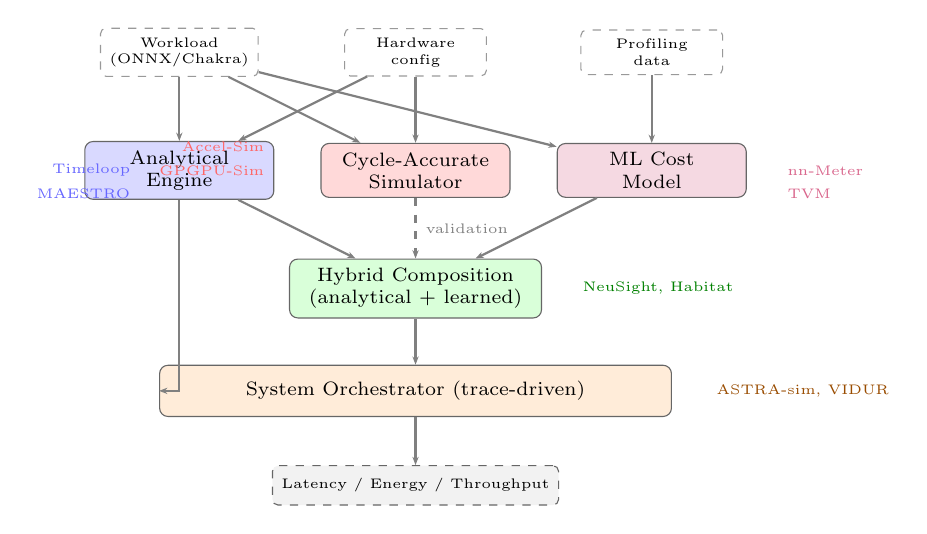
\begin{tikzpicture}[
    comp/.style={draw=black!60, rounded corners=3pt, minimum width=2.4cm, minimum height=0.65cm, align=center, font=\scriptsize},
    input/.style={draw=black!40, dashed, rounded corners=2pt, minimum width=1.8cm, minimum height=0.5cm, align=center, font=\tiny},
    arr/.style={-{Stealth[length=3pt]}, thick, black!50},
    lbl/.style={font=\tiny, text=black!50},
]

% Input layer
\node[input] (wl) at (0,4) {Workload\\(ONNX/Chakra)};
\node[input] (hw) at (3,4) {Hardware\\config};
\node[input] (prof) at (6,4) {Profiling\\data};

% Methodology layer
\node[comp, fill=blue!15] (analytical) at (0,2.5) {Analytical\\Engine};
\node[comp, fill=red!15] (simulator) at (3,2.5) {Cycle-Accurate\\Simulator};
\node[comp, fill=purple!15] (mlmodel) at (6,2.5) {ML Cost\\Model};

% Hybrid composition
\node[comp, fill=green!15, minimum width=3.2cm] (hybrid) at (3,1) {Hybrid Composition\\(analytical + learned)};

% System orchestration
\node[comp, fill=orange!15, minimum width=6.5cm] (system) at (3,-0.3) {System Orchestrator (trace-driven)};

% Output
\node[input, draw=black!60, fill=gray!10] (output) at (3,-1.5) {Latency / Energy / Throughput};

% Arrows - inputs to methods
\draw[arr] (wl) -- (analytical);
\draw[arr] (hw) -- (analytical);
\draw[arr] (hw) -- (simulator);
\draw[arr] (wl) -- (simulator);
\draw[arr] (prof) -- (mlmodel);
\draw[arr] (wl) -- (mlmodel);

% Arrows - methods to hybrid
\draw[arr] (analytical) -- (hybrid);
\draw[arr] (mlmodel) -- (hybrid);
\draw[arr, dashed, gray] (simulator) -- node[lbl, right] {validation} (hybrid);

% Arrows - to system
\draw[arr] (hybrid) -- (system);
\draw[arr] (analytical) |- (system);

% Arrows - output
\draw[arr] (system) -- (output);

% Example tools
\node[font=\tiny, text=blue!60, anchor=east] at (-0.5,2.5) {Timeloop};
\node[font=\tiny, text=blue!60, anchor=east] at (-0.5,2.2) {MAESTRO};
\node[font=\tiny, text=red!60, anchor=east] at (1.2,2.8) {Accel-Sim};
\node[font=\tiny, text=red!60, anchor=east] at (1.2,2.5) {GPGPU-Sim};
\node[font=\tiny, text=purple!60, anchor=west] at (7.6,2.5) {nn-Meter};
\node[font=\tiny, text=purple!60, anchor=west] at (7.6,2.2) {TVM};
\node[font=\tiny, text=green!50!black, anchor=west] at (5,1) {NeuSight, Habitat};
\node[font=\tiny, text=orange!60!black, anchor=west] at (6.7,-0.3) {ASTRA-sim, VIDUR};

\end{tikzpicture}%
}
\caption{Unified architecture showing how tool methodologies compose. Analytical engines and ML cost models feed into hybrid approaches, while system-level orchestrators (trace-driven) assemble component predictions into end-to-end estimates. Cycle-accurate simulators primarily serve as validation oracles.}
\label{fig:tool-architecture}
\end{figure}

\subsection{Primary Axis: Methodology Type}
\label{subsec:by-methodology}

The choice of methodology determines fundamental trade-offs between accuracy, evaluation speed, data requirements, and interpretability, as summarized in Table~\ref{tab:taxonomy-matrix}; Section~\ref{sec:survey} provides detailed per-tool analysis.

\textbf{Analytical models} (Timeloop~\cite{timeloop2019}: 5--10\% vs.\ RTL; MAESTRO~\cite{maestro2019}; Sparseloop~\cite{sparseloop2022}; AMALI~\cite{amali2025}) provide microsecond evaluation and full interpretability but require per-architecture derivation (AMALI's 23.6\% MAPE illustrates GPU dynamic effects).
\textbf{Cycle-accurate simulators} (GPGPU-Sim~\cite{gpgpusim2009}, Accel-Sim~\cite{accelsim2020}: 0.90--0.97 IPC; PyTorchSim~\cite{pytorchsim2025}) are impractical for DSE at $1000$--$10000\times$ slowdown~\cite{gpgpusim2009,accelsim2020}.
\textbf{Trace-driven simulators} (ASTRA-sim~\cite{astrasim2023}: 5--15\%; VIDUR~\cite{vidur2024}: $<$5\%; SimAI~\cite{simai2025}; Frontier~\cite{frontier2025}) replay execution traces for system-level modeling.
\textbf{ML-augmented models} (nn-Meter~\cite{nnmeter2021}; LitePred~\cite{litepred2024}; HELP~\cite{help2021}; TVM~\cite{tvm2018}/Ansor~\cite{ansor2020}) learn from profiling data but risk \emph{silent distribution shift}.
\textbf{Hybrid} approaches (NeuSight~\cite{neusight2025}: 2.3\% MAPE; Habitat~\cite{habitat2021}; ArchGym~\cite{archgym2023}) combine analytical priors with learned corrections~\cite{latencypredictorsnas2024}.

\subsection{Secondary Axes: Platform and Abstraction Level}
\label{subsec:by-platform}

Platform constrains methodology: \textbf{accelerators} use analytical models; \textbf{GPUs} span all types; \textbf{distributed systems} require trace-driven simulation; \textbf{edge devices} use ML-augmented approaches; \textbf{CPUs}~\cite{concorde2025,granite2022} are least studied.
Abstraction level determines composition errors (Figure~\ref{fig:abstraction-levels}): kernel-level tools achieve 2--3\% error, model-level 5--12\%, and system-level 5--15\%, with errors propagating through the chain.

\begin{figure}[t]
\centering
\resizebox{\columnwidth}{!}{%
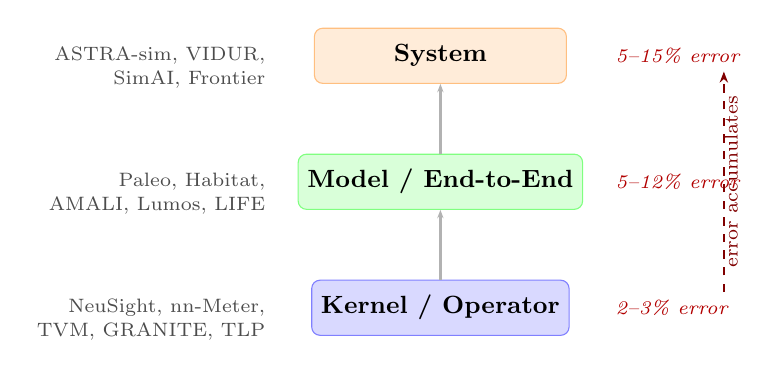
\begin{tikzpicture}[
  level/.style={draw, rounded corners=3pt, minimum width=3.2cm, minimum height=0.7cm, align=center, font=\small\bfseries},
  tool/.style={font=\scriptsize, text=black!70},
  err/.style={font=\scriptsize\itshape, text=red!70!black},
  arrow/.style={-{Stealth[length=3pt]}, thick, gray!60},
  compos/.style={-{Stealth[length=4pt]}, thick, red!50!black, dashed},
]

% Levels (bottom to top)
\node[level, fill=blue!15, draw=blue!50] (kernel) at (0,0) {Kernel / Operator};
\node[level, fill=green!15, draw=green!50] (model) at (0,1.6) {Model / End-to-End};
\node[level, fill=orange!15, draw=orange!50] (system) at (0,3.2) {System};

% Composition arrows between levels
\draw[arrow] (kernel) -- (model);
\draw[arrow] (model) -- (system);

% Tool names (left side)
\node[tool, anchor=east] at (-2.1,0) {NeuSight, nn-Meter,};
\node[tool, anchor=east] at (-2.1,-0.3) {TVM, GRANITE, TLP};
\node[tool, anchor=east] at (-2.1,1.6) {Paleo, Habitat,};
\node[tool, anchor=east] at (-2.1,1.3) {AMALI, Lumos, LIFE};
\node[tool, anchor=east] at (-2.1,3.2) {ASTRA-sim, VIDUR,};
\node[tool, anchor=east] at (-2.1,2.9) {SimAI, Frontier};

% Error ranges (right side)
\node[err, anchor=west] at (2.1,0) {2--3\% error};
\node[err, anchor=west] at (2.1,1.6) {5--12\% error};
\node[err, anchor=west] at (2.1,3.2) {5--15\% error};

% Composition problem annotation
\draw[compos] (3.6,0.2) -- (3.6,3.0);
\node[font=\scriptsize, text=red!50!black, rotate=90, anchor=south] at (3.9,1.6) {error accumulates};

\end{tikzpicture}%
}
\caption{Abstraction level hierarchy and the composition problem. Tools operate at one of three levels; composing predictions across levels accumulates error. Error ranges are representative values from surveyed papers.}
\label{fig:abstraction-levels}
\end{figure}

\subsection{Workload Coverage}
\label{subsec:workload-coverage}

Table~\ref{tab:workload-coverage} characterizes the workload types on which each tool has been validated, revealing a temporal validation lag rather than a methodological bias: tools published during the CNN-dominant era (2016--2022) naturally validated on the workloads of their time, while post-2023 tools increasingly target transformers and LLMs.

\begin{table}[t]
\centering
\caption{Workload validation coverage. \checkmark\ = validated in the original paper; $\circ$ = partial or indirect validation; --- = no validation.
Nearly all tools report accuracy on CNN workloads; transformer and MoE coverage is sparse.
Empty columns (diffusion, dynamic inference) represent workload types with \emph{no} validated performance modeling tools.}
\label{tab:workload-coverage}
\small
\begin{tabular}{lccccc}
\toprule
 & & \textbf{Trans-} & \textbf{LLM} & & \\
\textbf{Tool} & \textbf{CNN} & \textbf{former} & \textbf{Train} & \textbf{MoE} & \textbf{Diff.} \\
\midrule
Timeloop & \checkmark & $\circ$ & --- & --- & --- \\
MAESTRO & \checkmark & --- & --- & --- & --- \\
NeuSight & \checkmark & \checkmark & --- & --- & --- \\
Habitat & \checkmark & --- & --- & --- & --- \\
AMALI & --- & \checkmark & --- & --- & --- \\
ASTRA-sim & \checkmark & $\circ$ & \checkmark & --- & --- \\
VIDUR & --- & \checkmark & --- & --- & --- \\
SimAI & --- & --- & \checkmark & --- & --- \\
Lumos & --- & --- & \checkmark & --- & --- \\
Frontier & --- & \checkmark & --- & \checkmark & --- \\
nn-Meter & \checkmark & --- & --- & --- & --- \\
LitePred & \checkmark & --- & --- & --- & --- \\
HELP & \checkmark & --- & --- & --- & --- \\
TVM/Ansor & \checkmark & $\circ$ & --- & --- & --- \\
\bottomrule
\end{tabular}
\end{table}

Figure~\ref{fig:validation-bias} quantifies this temporal validation lag: of the 14 surveyed tools, 9 (64\%) include CNN validation, reflecting the dominance of CNNs when those tools were published.
Critically, the lag is closing---post-2023 tools (VIDUR, Frontier, Lumos, SimAI) validate exclusively on transformers/LLMs---but emerging workloads remain uncovered: \textbf{no surveyed tool has been validated on diffusion models or dynamic inference workloads}~\cite{dynamicreasoning2026}, only Frontier~\cite{frontier2025} has validated MoE support, and no single tool offers validated transformer prediction across the full kernel-to-system stack.
The practical consequence: practitioners working with frontier workloads must accept unvalidated predictions, collect their own validation data, or fall back to measurement.

\begin{figure}[t]
\centering
\resizebox{0.85\columnwidth}{!}{%
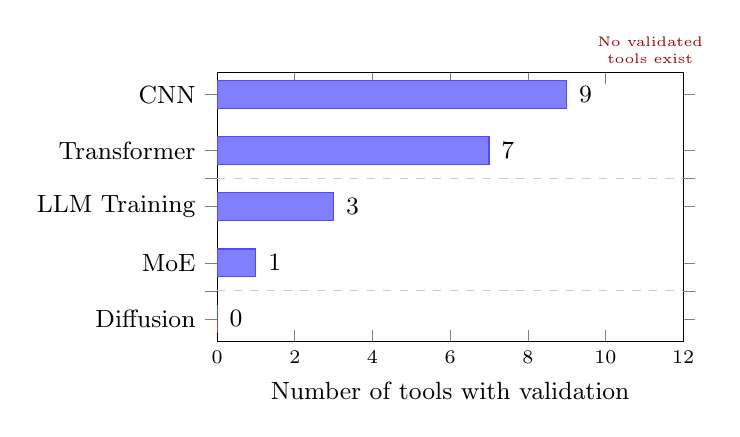
\begin{tikzpicture}
\begin{axis}[
    xbar,
    y dir=reverse,
    xlabel={Number of tools with validation},
    xmin=0, xmax=12,
    ytick={0,1,2,3,4},
    yticklabels={CNN, Transformer, LLM Training, MoE, Diffusion},
    yticklabel style={font=\small},
    xticklabel style={font=\scriptsize},
    xlabel style={font=\small},
    bar width=10pt,
    height=5cm,
    width=7.5cm,
    nodes near coords,
    nodes near coords style={font=\small\bfseries, anchor=west},
    every node near coord/.append style={xshift=1pt},
    extra y ticks={1.5, 3.5},
    extra y tick labels={},
    extra y tick style={grid=major, grid style={black!20, dashed}},
]
\addplot[fill=blue!50, draw=blue!70] coordinates {(9,0) (7,1) (3,2) (1,3) (0,4)};
\end{axis}
% Annotation
\node[font=\tiny, text=red!60!black, align=center] at (5.5,3.7) {No validated\\tools exist};
\end{tikzpicture}%
}
\caption{Workload validation coverage across surveyed tools. CNN validation reflects the temporal publication distribution (most tools published 2016--2022), while MoE and diffusion models---dominant only since 2023---have minimal or no validated prediction tools.}
\label{fig:validation-bias}
\end{figure}

% ==============================================================================
% SURVEY OF APPROACHES
% ==============================================================================
\section{Survey of Approaches}
\label{sec:survey}

This section surveys performance modeling tools for ML workloads, organized by target platform, examining modeling challenges, available tools, and their strengths and limitations.
Table~\ref{tab:survey-summary} provides a comprehensive comparison.

\begin{table*}[t]
\centering
\caption{Summary of surveyed performance modeling tools for ML workloads, organized by target platform. \textbf{Methodology}: A=Analytical, S=Simulation, T=Trace-driven, M=ML-augmented, H=Hybrid. $^*$Accuracy measures surrogate-vs-simulator fidelity, not real hardware error. $^\dagger$Reported accuracy unverifiable due to reproducibility issues. $^\ddagger$No accuracy baseline against real hardware reported.}
\label{tab:survey-summary}
\small
\begin{tabular}{lllllll}
\toprule
\textbf{Tool} & \textbf{Platform} & \textbf{Method} & \textbf{Target} & \textbf{Accuracy} & \textbf{Speed} & \textbf{Key Capability} \\
\midrule
\multicolumn{7}{l}{\textit{DNN Accelerator Modeling}} \\
Timeloop~\cite{timeloop2019} & NPU & A & Latency/Energy & 5--10\% & $\mu$s & Loop-nest DSE \\
MAESTRO~\cite{maestro2019} & NPU & A & Latency/Energy & 5--15\% & $\mu$s & Data-centric directives \\
Sparseloop~\cite{sparseloop2022} & NPU & A & Sparse tensors & 5--10\% & $\mu$s & Compression modeling \\
PyTorchSim~\cite{pytorchsim2025} & NPU & S & Cycle-accurate & N/A$^\ddagger$ & Hours & PyTorch 2 integration \\
ArchGym~\cite{archgym2023} & Multi & H & Multi-objective & 0.61\%$^*$ & ms & ML-aided DSE \\
\midrule
\multicolumn{7}{l}{\textit{GPU Performance Modeling}} \\
Accel-Sim~\cite{accelsim2020} & GPU & S & Cycle-accurate & 10--20\% & Hours & SASS trace-driven \\
GPGPU-Sim~\cite{gpgpusim2009} & GPU & S & Cycle-accurate & 10--20\% & Hours & CUDA workloads \\
AMALI~\cite{amali2025} & GPU & A & LLM inference & 23.6\% & ms & Memory hierarchy \\
NeuSight~\cite{neusight2025} & GPU & H & Kernel/E2E latency & 2.3\% & ms & Tile-based prediction \\
Habitat~\cite{habitat2021} & GPU & H & Training time & 11.8\% & Per-kernel & Wave scaling \\
\midrule
\multicolumn{7}{l}{\textit{Distributed Training and LLM Serving}} \\
ASTRA-sim~\cite{astrasim2023} & Distributed & T & Training time & 5--15\% & Minutes & Collective modeling \\
SimAI~\cite{simai2025} & Distributed & T & Training time & 1.9\% & Minutes & Full-stack simulation \\
Lumos~\cite{lumos2025} & Distributed & T & LLM training & 3.3\% & Minutes & H100 training \\
VIDUR~\cite{vidur2024} & GPU cluster & T & LLM serving & $<$5\% & Seconds & Prefill/decode phases \\
Frontier~\cite{frontier2025} & Distributed & T & MoE inference & --- & Minutes & Stage-centric sim. \\
TrioSim~\cite{triosim2025} & Multi-GPU & T & DNN training & N/A$^\ddagger$ & Minutes & Lightweight multi-GPU \\
\midrule
\multicolumn{7}{l}{\textit{Edge Device Modeling}} \\
nn-Meter~\cite{nnmeter2021} & Edge & M & Latency & $<$1\%$^\dagger$ & ms & Kernel detection \\
LitePred~\cite{litepred2024} & Edge & M & Latency & 0.7\% & ms & 85-platform transfer \\
HELP~\cite{help2021} & Multi & M & Latency & 1.9\% & ms & 10-sample adaptation \\
\midrule
\multicolumn{7}{l}{\textit{Compiler Cost Models}} \\
TVM~\cite{tvm2018} & GPU & M & Schedule perf. & $\sim$15\% & ms & Autotuning guidance \\
Ansor~\cite{ansor2020} & GPU & M & Schedule perf. & $\sim$15\% & ms & Program sampling \\
TLP~\cite{tlp2023} & GPU & M & Tensor program & $<$10\% & ms & Transformer cost model \\
\bottomrule
\end{tabular}
\end{table*}

\subsection{DNN Accelerator Modeling}
\label{subsec:accelerator-modeling}

The analytical tractability of DNN accelerator modeling stems from the regularity of computation~\cite{sze2017efficient}, building on early characterization pioneered by DianNao~\cite{diannao2014}.
A convolution layer maps to a seven-deep nested loop over batch, output channel, input channel, and spatial dimensions; Timeloop~\cite{timeloop2019} enumerates mappings of these loops to a spatial-temporal hardware hierarchy, computing data reuse at each memory level as the ratio of loop bounds.
This exhaustive search finds the optimal dataflow in microseconds (5--10\% error, $2000\times$ speedup) because the search space, though combinatorially large, admits efficient pruning: any mapping that exceeds a memory level's capacity is immediately discarded.
MAESTRO~\cite{maestro2019} achieves similar modeling with a more compact ``data-centric'' representation that specifies which data dimension is stationary at each level, trading enumeration completeness for specification simplicity---but sacrificing Timeloop's ability to model per-PE utilization, explaining why Timeloop achieves tighter error bounds on architectures with irregular PE arrays.
SCALE-Sim~\cite{scalesim2019} complements both by providing cycle-accurate systolic array simulation for validation.
Sparseloop~\cite{sparseloop2022} extends Timeloop's analysis to sparse tensors by introducing format-specific access count models for compression formats (CSR, bitmap)---the key challenge being that sparse data access patterns depend on the data values, requiring statistical or format-aware modeling rather than purely geometric analysis.
PyTorchSim~\cite{pytorchsim2025} integrates PyTorch~2 with NPU simulation but lacks real-hardware validation; ArchGym~\cite{archgym2023} connects ML surrogates to simulators (0.61\% RMSE vs.\ simulator, not hardware).
Accelerator modeling is the most mature subdomain, with Timeloop as the de facto DSE standard. The key gap is silicon validation; emerging PIM tools~\cite{upimulator2024,attacc2024,neupims2024,paise2025} also lack hardware validation.

\subsection{GPU Performance Modeling}
\label{subsec:gpu-modeling}

GPUs dominate ML training and inference, requiring models for SIMT execution, warp scheduling, memory coalescing, and occupancy effects.

\textbf{Cycle-accurate simulation.}
GPGPU-Sim~\cite{gpgpusim2009} and Accel-Sim~\cite{accelsim2020} achieve 0.90--0.97 IPC correlation but at $1000$--$10000\times$ slowdown; reverse-engineering~\cite{dissectinggpu2025} improved Accel-Sim to 13.98\% MAPE.
These simulators integrate with memory subsystem models---from DRAMSim2~\cite{dramsim2_2011} and Ramulator~\cite{ramulator2015} to their modern successors DRAMSim3~\cite{dramsim3_2020} and Ramulator~2.0~\cite{ramulator2_2023}---for accurate DRAM timing, critical for memory-bound LLM inference.

\textbf{Analytical and hybrid models.}
AMALI~\cite{amali2025} models GPU performance through memory hierarchy analysis (L1, L2, HBM data movement volumes); the roofline model~\cite{williams2009roofline} provides upper bounds, with recent LLM-specific extensions~\cite{rooflinellm2024}.
NeuSight~\cite{neusight2025} achieves 2.3\% MAPE on GPT-3 kernels by decomposing each kernel into \emph{tiles} corresponding 1:1 with CUDA thread blocks.
This abstraction succeeds because GPU scheduling is tile-based: each SM's execution time depends on arithmetic intensity, shared memory footprint, and register pressure---all locally measurable per tile.
By profiling representative tiles and extrapolating via occupancy, NeuSight captures memory bandwidth saturation and L2 cache pressure without modeling warp scheduling details.
AMALI's whole-kernel model misses these effects by averaging data movement over the entire kernel, losing per-SM occupancy information.
Habitat~\cite{habitat2021} achieves 11.8\% cross-GPU transfer via wave scaling based on SM count and memory bandwidth ratios.

The accuracy disparity reflects a fundamental distinction: accelerator execution is deterministic (loop nests fully determine data movement), while GPUs introduce warp scheduling, memory coalescing, and L2 cache contention that progressively degrade analytical accuracy.

\textbf{LLM-specific and compiler models.}
VIDUR~\cite{vidur2024} simulates LLM serving at $<$5\% error; LIFE~\cite{life2025}, HERMES~\cite{hermes2025}, Omniwise~\cite{omniwise2025}, and SwizzlePerf~\cite{swizzleperf2025} target inference.
TVM~\cite{tvm2018}/Ansor~\cite{ansor2020} ($\sim$15\% MAPE), TLP~\cite{tlp2023} ($<$10\%), and SynPerf~\cite{synperf2025} target compiler autotuning~\cite{tenset2021}.

\subsection{Distributed Training and LLM Serving}
\label{subsec:distributed-modeling}

Distributed systems require modeling communication, synchronization, and parallelism strategies~\cite{megatronlm2020,gpipe2019,zero2020}.
ASTRA-sim~\cite{astrasim2023} achieves 5--15\% error via Chakra traces~\cite{chakra2023}; SimAI~\cite{simai2025} reaches 1.9\% at Alibaba scale; Echo~\cite{echo2024} scales simulation to 10K+ devices; Lumos~\cite{lumos2025} 3.3\% on H100s; PRISM~\cite{prism2025} provides prediction intervals at 10K+ GPUs.
Paleo~\cite{paleo2017} pioneered analytical estimation; MAD Max~\cite{madmax2024} and Sailor~\cite{sailor2025} extend it; Llama~3~\cite{llama3scaling2025} provides validation ground truth at 16K GPUs.
The speed--fidelity hierarchy among these simulators reflects fundamentally different modeling granularities.
VIDUR models serving at the \emph{request level}: each prefill/decode phase is a single event with profiled duration, yielding second-scale simulation.
ASTRA-sim operates at the \emph{collective communication level}, replaying Chakra traces~\cite{chakra2023} to model compute-communication overlap critical for training.
SimAI decomposes further to the \emph{NCCL algorithm level}, modeling chunk-based ring/tree reductions---this matters because network congestion is non-linear: overlapping collectives that individually fit within bandwidth may congest, an effect invisible to per-collective models.
SimAI's 1.9\% MAPE (vs.\ ASTRA-sim's 5--15\%) reflects this fidelity gain at production scale, though Echo~\cite{echo2024} shows the cost: lightweight modeling is needed to scale to 10K+ devices.

For inference serving, VIDUR~\cite{vidur2024} models scheduling with vLLM~\cite{vllm2023}; DistServe~\cite{distserve2024} disaggregates prefill and decode for goodput optimization; Frontier~\cite{frontier2025} targets MoE; POD-Attention~\cite{podattention2025} and AQUA~\cite{aqua2025} address prefill-decode overlap and memory offloading respectively; ThrottLL'eM~\cite{throttllem2025} models power effects; speculative decoding~\cite{medusa2024} creates a moving target for all simulators.

\subsection{Edge Device Modeling}
\label{subsec:edge-modeling}

Hardware diversity makes per-device analytical modeling impractical.
nn-Meter~\cite{nnmeter2021} claims $<$1\% MAPE but is unverifiable due to dependency failures (Section~\ref{sec:evaluation}); LitePred~\cite{litepred2024} achieves 0.7\% across 85 platforms; HELP~\cite{help2021} reaches 1.9\% with 10-sample meta-learning.
ESM~\cite{esm2025} finds well-tuned random forests match deep learning surrogates, and transfer learning provides 22.5\% improvement~\cite{latencypredictorsnas2024}---suggesting data quality matters more than model sophistication.

\subsection{Cross-Cutting Themes}
\label{subsec:cross-cutting}

Three architectural insights emerge.
\emph{First}, structural decomposition aligned with hardware execution boundaries consistently outperforms black-box approaches: Timeloop's loop nests reflect systolic array dataflow, NeuSight's tiles mirror CUDA thread block scheduling, and VIDUR's prefill/decode split captures distinct compute- vs.\ memory-bound regimes.
\emph{Second}, the critical modeling features differ by platform: data reuse for accelerators, thread block occupancy for GPUs, and collective topology for distributed systems---explaining why no single methodology spans all platforms.
\emph{Third}, a persistent \textbf{accuracy--generality--speed trade-off} drives methodological diversity; subdomain maturity correlates with economic incentive: accelerator DSE is most mature (irreversible chip errors), distributed training is fastest-growing (million-dollar runs), and edge modeling has weakest reproducibility.

% ==============================================================================
% COMPARISON AND ANALYSIS
% ==============================================================================
\section{Comparison and Analysis}
\label{sec:comparison}

We analyze trade-offs across methodology types along accuracy and speed dimensions (see Table~\ref{tab:survey-summary} for per-tool details); generalization and interpretability challenges are deferred to Section~\ref{sec:challenges}.
Figure~\ref{fig:accuracy-speed} visualizes the accuracy--speed trade-off space.

\textbf{Caveat.}
The accuracy values in Figures~\ref{fig:accuracy-speed} and~\ref{fig:accuracy-comparison} are \emph{self-reported} on each tool's own benchmarks and hardware.
No common evaluation benchmark exists for performance modeling tools, so these numbers are \textbf{not directly comparable across platforms or workload types}.
We include them to illustrate \emph{within-domain} trade-offs and identify difficult problem domains, not to rank tools against each other.
A common-benchmark comparison is a key future direction (Section~\ref{sec:challenges}).

\begin{figure}[t]
\centering
\resizebox{\columnwidth}{!}{%
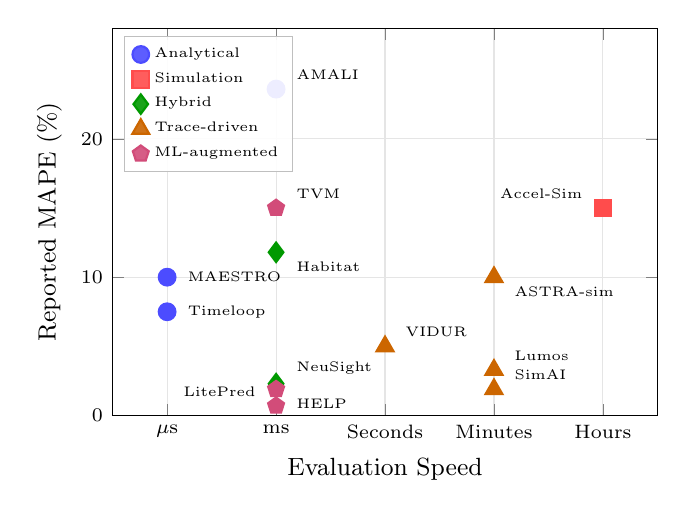
\begin{tikzpicture}
\begin{axis}[
    xlabel={Evaluation Speed},
    ylabel={Reported MAPE (\%)},
    ymin=0, ymax=28,
    xmin=-0.5, xmax=4.5,
    xtick={0,1,2,3,4},
    xticklabels={$\mu$s, ms, Seconds, Minutes, Hours},
    xticklabel style={font=\scriptsize},
    yticklabel style={font=\scriptsize},
    xlabel style={font=\small},
    ylabel style={font=\small},
    height=6.5cm,
    width=8.5cm,
    grid=both,
    grid style={gray!20},
    legend style={at={(0.02,0.98)}, anchor=north west, font=\tiny, draw=gray!50, fill=white, fill opacity=0.9, text opacity=1},
    legend cell align={left},
]
% Analytical (blue circles)
\addplot[only marks, mark=*, mark size=3pt, blue!70, thick] coordinates {(0,7.5) (0,10) (1,23.6)};
% Simulation (red squares)
\addplot[only marks, mark=square*, mark size=3pt, red!70, thick] coordinates {(4,15)};
% Hybrid (green diamonds)
\addplot[only marks, mark=diamond*, mark size=3.5pt, green!60!black, thick] coordinates {(1,2.3) (1,11.8)};
% Trace-driven (orange triangles)
\addplot[only marks, mark=triangle*, mark size=3.5pt, orange!80!black, thick] coordinates {(2,5) (3,1.9) (3,3.3) (3,10)};
% ML-augmented (purple pentagons)
\addplot[only marks, mark=pentagon*, mark size=3pt, purple!70, thick] coordinates {(1,0.7) (1,1.9) (1,15)};
% Labels
\node[font=\tiny, anchor=west] at (0.1,7.5) {Timeloop};
\node[font=\tiny, anchor=west] at (0.1,10) {MAESTRO};
\node[font=\tiny, anchor=south west] at (1.1,23.6) {AMALI};
\node[font=\tiny, anchor=south east] at (3.9,15) {Accel-Sim};
\node[font=\tiny, anchor=south west] at (1.1,2.3) {NeuSight};
\node[font=\tiny, anchor=north west] at (1.1,11.8) {Habitat};
\node[font=\tiny, anchor=south west] at (2.1,5) {VIDUR};
\node[font=\tiny, anchor=south west] at (3.1,1.9) {SimAI};
\node[font=\tiny, anchor=south west] at (3.1,3.3) {Lumos};
\node[font=\tiny, anchor=north west] at (3.1,10) {ASTRA-sim};
\node[font=\tiny, anchor=south east] at (0.9,0.7) {LitePred};
\node[font=\tiny, anchor=north west] at (1.1,1.9) {HELP};
\node[font=\tiny, anchor=south west] at (1.1,15) {TVM};
\legend{Analytical, Simulation, Hybrid, Trace-driven, ML-augmented}
\end{axis}
\end{tikzpicture}%
}
\caption{Self-reported accuracy vs.\ evaluation speed across surveyed tools. Each point represents a tool's MAPE on its \emph{own} benchmarks and hardware---values are not directly comparable across tools targeting different platforms. The dashed line is an approximate visual guide, not a true Pareto frontier.}
\label{fig:accuracy-speed}
\end{figure}

\subsection{Accuracy by Problem Difficulty}
\label{subsec:accuracy-difficulty}

We organize accuracy results by inherent problem difficulty rather than comparing across incompatible benchmarks (Figure~\ref{fig:accuracy-comparison}).
Accelerator modeling is most tractable (5--10\%) due to deterministic data movement; GPU kernel prediction achieves 2--12\% via hybrid methods; distributed systems reach 2--15\% where communication modeling dominates error; edge prediction achieves 0.7--2\% but requires per-device profiling.
The architectural reasons for these difficulty tiers are analyzed in Sections~\ref{subsec:gpu-modeling} and~\ref{subsec:distributed-modeling}.

\begin{figure}[t]
\centering
\resizebox{\columnwidth}{!}{%
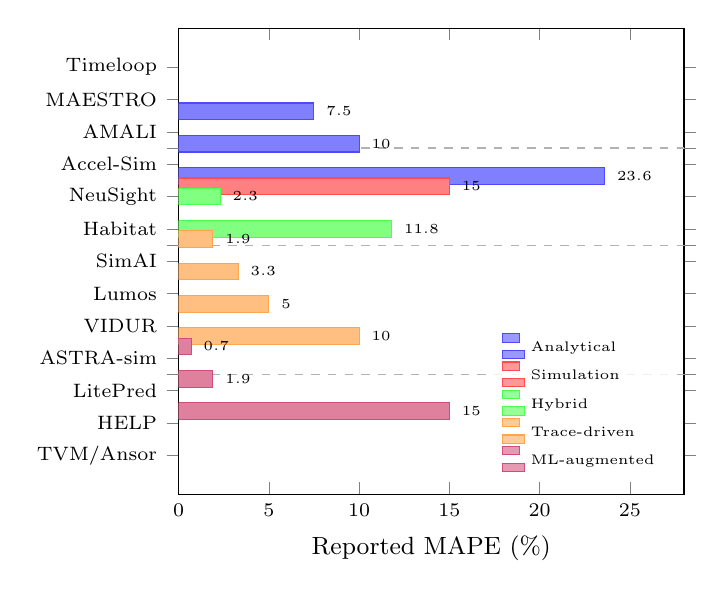
\begin{tikzpicture}
\begin{axis}[
    xbar,
    y dir=reverse,
    xlabel={Reported MAPE (\%)},
    xmin=0, xmax=28,
    ytick={0,1,2,3,4,5,6,7,8,9,10,11,12},
    yticklabels={
        Timeloop,
        MAESTRO,
        AMALI,
        Accel-Sim,
        NeuSight,
        Habitat,
        SimAI,
        Lumos,
        VIDUR,
        ASTRA-sim,
        LitePred,
        HELP,
        TVM/Ansor
    },
    yticklabel style={font=\scriptsize},
    xticklabel style={font=\scriptsize},
    xlabel style={font=\small},
    bar width=6pt,
    height=7.5cm,
    width=8cm,
    nodes near coords,
    nodes near coords style={font=\tiny, anchor=west},
    every node near coord/.append style={xshift=1pt},
    legend style={at={(0.97,0.03)}, anchor=south east, font=\tiny, draw=none, fill=white, fill opacity=0.8, text opacity=1},
    legend cell align={left},
    extra y ticks={2.5, 5.5, 9.5},
    extra y tick labels={},
    extra y tick style={grid=major, grid style={black!30, dashed}},
]
% Analytical (blue)
\addplot[fill=blue!50, draw=blue!70] coordinates {(7.5,0) (10,1) (23.6,2)};
% Simulation (red)
\addplot[fill=red!50, draw=red!70] coordinates {(15,3)};
% Hybrid (green)
\addplot[fill=green!50, draw=green!70] coordinates {(2.3,4) (11.8,5)};
% Trace-driven (orange)
\addplot[fill=orange!50, draw=orange!70] coordinates {(1.9,6) (3.3,7) (5,8) (10,9)};
% ML-augmented (purple)
\addplot[fill=purple!50, draw=purple!70] coordinates {(0.7,10) (1.9,11) (15,12)};
\legend{Analytical, Simulation, Hybrid, Trace-driven, ML-augmented}
\end{axis}
\end{tikzpicture}%
}
\caption{Self-reported accuracy (MAPE) of surveyed tools, grouped by methodology type. Range midpoints used where ranges are reported. \textbf{Values are not directly comparable} across tools: each was measured on different benchmarks, workloads, and hardware. Horizontal groupings by dashed lines separate distinct problem domains (accelerator, GPU, distributed, edge).}
\label{fig:accuracy-comparison}
\end{figure}

\subsection{Practitioner Tool Selection}
\label{subsec:tool-selection}

Tool selection depends on target platform and acceptable error margin.
Accelerator DSE: Timeloop/MAESTRO ($\mu$s-speed); Sparseloop for sparse workloads.
GPU: NeuSight for accuracy--speed balance; Accel-Sim for $\mu$arch detail.
Distributed: VIDUR for serving; ASTRA-sim/SimAI for training at scale.
Edge: LitePred for coverage; HELP with minimal data.
Additional factors include available hardware for profiling, team expertise with specific frameworks, integration with existing workflows, and license constraints.
Prefer Docker-first tools (Section~\ref{sec:evaluation}).

% ==============================================================================
% EXPERIMENTAL EVALUATION
% ==============================================================================
\section{Experimental Evaluation}
\label{sec:evaluation}

We conducted hands-on evaluations of five tools spanning methodology types: Timeloop (analytical), ASTRA-sim (trace-driven, distributed), VIDUR (trace-driven, LLM serving), nn-Meter (ML-augmented, edge), and NeuSight (hybrid, GPU).
We selected one tool per methodology type to maximize coverage; we excluded proprietary tools (e.g., NVIDIA Nsight Compute, internal TPU profilers) as they cannot be independently reproduced.

\textbf{Scope and limitations.}
All evaluations ran on Apple M2 Ultra (aarch64, 192\,GB RAM) using Docker containers where provided.
\emph{No GPU hardware was available}, so we \textbf{do not validate accuracy claims}.
Instead, we evaluate \emph{reproducibility}: can a practitioner reproduce a tool's functionality without the original authors' environment?
This complements accuracy evaluation, which would require common-benchmark runs on target hardware (Section~\ref{sec:challenges}).
Table~\ref{tab:evaluation-summary} summarizes results.

\begin{table}[t]
\centering
\caption{Reproducibility evaluation results (not accuracy evaluation). Scores reflect setup ease, output consistency, and usability---not prediction accuracy, which would require target hardware. $^\dagger$Timeloop CLI works but Python bindings fail.}
\label{tab:evaluation-summary}
\small
\begin{tabular}{lcccc}
\toprule
\textbf{Tool} & \textbf{Setup} & \textbf{Reprod.} & \textbf{Usability} & \textbf{Total} \\
\midrule
VIDUR & 2.5 & 3.5 & 3 & 9/10 \\
Timeloop$^\dagger$ & 3 & 4 & 2 & 9/10 \\
ASTRA-sim & 2.5 & 3 & 3 & 8.5/10 \\
NeuSight & 2 & 3 & 2.5 & 7.5/10 \\
nn-Meter & 2 & 0 & 1 & 3/10 \\
\bottomrule
\end{tabular}
\end{table}

\subsection{Per-Tool Results}
\label{subsec:per-tool-results}

\textbf{VIDUR} (9/10).
We simulated Llama-2-7B on a simulated A100 (Table~\ref{tab:vidur-results}).
The simulator's outputs are internally consistent with expected scheduler behavior: Sarathi shows 12.2\% lower simulated latency than vLLM (consistent with chunked prefill~\cite{sarathi2024}); vLLM preempted 26.5\% of requests vs.\ zero for Sarathi, reflecting KV-cache management differences~\cite{vllm2023}.
These confirm VIDUR produces plausible outputs, though ground-truth validation would require running the same configurations on real A100 hardware.

\begin{table}[t]
\centering
\caption{VIDUR simulation results for Llama-2-7B inference serving on a simulated A100 GPU. All metrics from our own experiments.}
\label{tab:vidur-results}
\small
\begin{tabular}{lcc}
\toprule
\textbf{Metric} & \textbf{vLLM} & \textbf{Sarathi} \\
\midrule
Requests & 200 & 50 \\
Avg E2E latency (s) & 0.177 & 0.158 \\
P99 E2E latency (s) & 0.320 & 0.270 \\
Avg TTFT (s) & 0.027 & 0.025 \\
Avg TPOT (s) & 0.0093 & 0.0090 \\
Requests preempted & 53 & 0 \\
\bottomrule
\end{tabular}
\end{table}

\textbf{Timeloop} (9/10).
Docker CLI produces deterministic, bit-identical outputs for Eyeriss-like configurations; reference outputs enable hardware-free verification.
Python bindings fail (\texttt{ImportError: libbarvinok.so.23}).

\textbf{ASTRA-sim} (8.5/10).
We ran collective microbenchmarks and ResNet-50 training at 2--8 simulated GPUs (Table~\ref{tab:astrasim-results}).
Internal consistency checks pass: Reduce-Scatter takes half the time of All-Reduce (consistent with half the data volume); communication overhead scales 5.76$\times$ for 4$\times$ more GPUs, matching ring All-Reduce complexity.
Our small-scale tests (2--8 GPUs) probe only the simulator's basic functionality; production-scale validation at 100+ GPUs---where network congestion effects dominate---would be needed to assess accuracy under realistic conditions.

\begin{table}[t]
\centering
\caption{ASTRA-sim quantitative results from our experiments on the HGX-H100 configuration. Top: collective microbenchmarks (8 NPUs, 1\,MB). Bottom: ResNet-50 data-parallel training scaling.}
\label{tab:astrasim-results}
\small
\begin{tabular}{lrr}
\toprule
\multicolumn{3}{l}{\textbf{Collective Microbenchmarks (8 NPUs, 1\,MB)}} \\
\midrule
\textbf{Collective} & \textbf{Cycles} & \textbf{Ratio vs.\ AR} \\
\midrule
All-Reduce & 57,426 & 1.000 \\
All-Gather & 44,058 & 0.767 \\
Reduce-Scatter & 28,950 & 0.504 \\
All-to-All & 114,000 & 1.985 \\
\midrule
\multicolumn{3}{l}{\textbf{ResNet-50 Data-Parallel Training}} \\
\midrule
\textbf{GPUs} & \textbf{Comm Cycles} & \textbf{Comm Overhead} \\
\midrule
2 & 574,289 & 0.05\% \\
4 & 1,454,270 & 0.13\% \\
8 & 3,307,886 & 0.30\% \\
\bottomrule
\end{tabular}
\end{table}

\textbf{NeuSight} (7.5/10).
Tile-based decomposition mirrors CUDA tiling for dense operations; irregular workloads had limited examples.

\textbf{nn-Meter} (3/10).
After four attempts ($>$4h), no predictions ran: pickle-serialized predictors (scikit-learn 0.23.1) are incompatible with current versions. The claimed $<$1\% MAPE is \textbf{unverifiable}.

Figure~\ref{fig:reproducibility-scores} visualizes the reproducibility assessment, showing that Docker-first tools are consistently easier to reproduce.

\begin{figure}[t]
\centering
\resizebox{\columnwidth}{!}{%
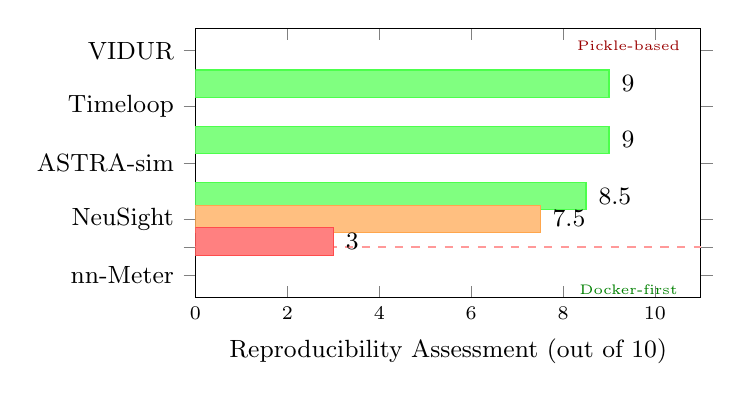
\begin{tikzpicture}
\begin{axis}[
    xbar,
    y dir=reverse,
    xlabel={Reproducibility Assessment (out of 10)},
    xmin=0, xmax=11,
    ytick={0,1,2,3,4},
    yticklabels={VIDUR, Timeloop, ASTRA-sim, NeuSight, nn-Meter},
    yticklabel style={font=\small},
    xticklabel style={font=\scriptsize},
    xlabel style={font=\small},
    bar width=10pt,
    height=5cm,
    width=8cm,
    nodes near coords,
    nodes near coords style={font=\small\bfseries, anchor=west},
    every node near coord/.append style={xshift=1pt},
    extra y ticks={3.5},
    extra y tick labels={},
    extra y tick style={grid=major, grid style={red!40, thick, dashed}},
]
% Docker-first tools (green)
\addplot[fill=green!50, draw=green!70] coordinates {(9,0) (9,1) (8.5,2)};
% Non-Docker tools (red)
\addplot[fill=orange!50, draw=orange!70] coordinates {(7.5,3)};
\addplot[fill=red!50, draw=red!70] coordinates {(3,4)};
\end{axis}
% Annotations
\node[font=\tiny, text=green!50!black, align=center] at (5.5,0.1) {Docker-first};
\node[font=\tiny, text=red!60!black, align=center] at (5.5,3.2) {Pickle-based};
\end{tikzpicture}%
}
\caption{Reproducibility assessment for evaluated tools. Docker-first tools (VIDUR, Timeloop, ASTRA-sim) are consistently reproducible, while tools relying on serialized ML models (nn-Meter) become unusable. The dashed line separates Docker-based from non-Docker deployments.}
\label{fig:reproducibility-scores}
\end{figure}

\subsection{Lessons and Threats to Validity}
\label{subsec:eval-lessons}

Key lessons:
(1)~Docker-first deployment correlates with reproducibility (all three Docker tools succeeded; nn-Meter without Docker failed), though our sample is small.
(2)~ML model serialization is fragile---nn-Meter's pickle predictors became unusable within two years.
(3)~Reference outputs enable trust without hardware (Timeloop, ASTRA-sim).
(4)~Scale-limited evaluation understates system tools---our 2--8 GPU tests are far below production scale~\cite{llama3scaling2025}.

\textbf{Threats.}
Our venue-focused search may under-represent industry and non-English publications.
We exclude proprietary tools (Nsight Compute~\cite{nsightcompute2019}, internal TPU models) from evaluation, though these are among the most widely used in practice; Section~\ref{sec:methodology} discusses their relationship to surveyed tools.
Accuracy metrics vary across papers (MAPE, RMSE, Kendall's $\tau$), limiting direct comparison---we explicitly caveat all cross-tool comparisons (Figures~\ref{fig:accuracy-speed},~\ref{fig:accuracy-comparison}).
Our evaluation covers only 5 of 22 tools, selected for methodology diversity rather than representativeness; a more complete study would include SimAI, AMALI, and Habitat.

% ==============================================================================
% OPEN CHALLENGES
% ==============================================================================
\section{Open Challenges and Future Directions}
\label{sec:challenges}

\textbf{Generalization gaps.}
\emph{Workload}: The temporal validation lag (Section~\ref{sec:taxonomy}) is closing for transformers but remains wide for emerging workloads---MoE, diffusion~\cite{dynamicreasoning2026}, and dynamic inference lack validated tools; scaling laws~\cite{kaplan2020scaling,hoffmann2022chinchilla,scalinglaws2024,scalinglawguide2025} predict loss but not latency.
Figure~\ref{fig:workload-coverage} shows the shift toward LLM workloads since 2023.
\emph{Hardware}: cross-family transfer (GPU$\rightarrow$TPU$\rightarrow$PIM) remains unsolved despite meta-learning (HELP) and feature-based transfer (LitePred).
\emph{Temporal}: software stack evolution silently invalidating models is addressed by no tool.

\begin{figure}[t]
\centering
\resizebox{\columnwidth}{!}{%
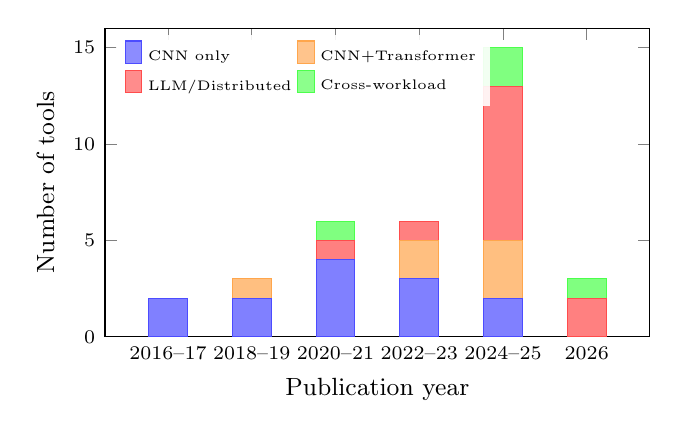
\begin{tikzpicture}
\begin{axis}[
    ybar stacked,
    bar width=14pt,
    xlabel={Publication year},
    ylabel={Number of tools},
    ymin=0, ymax=16,
    xtick={2016,2018,2020,2022,2024,2026},
    xticklabels={2016--17,2018--19,2020--21,2022--23,2024--25,2026},
    xticklabel style={font=\scriptsize},
    yticklabel style={font=\scriptsize},
    xlabel style={font=\small},
    ylabel style={font=\small},
    legend style={at={(0.02,0.98)}, anchor=north west, font=\tiny, draw=none, fill=white, fill opacity=0.9, text opacity=1, legend columns=2},
    legend cell align={left},
    height=5.5cm,
    width=8.5cm,
    enlarge x limits={abs=0.8cm},
]
\addplot[fill=blue!50, draw=blue!70] coordinates {(2016,2) (2018,2) (2020,4) (2022,3) (2024,2) (2026,0)};
\addplot[fill=orange!50, draw=orange!70] coordinates {(2016,0) (2018,1) (2020,0) (2022,2) (2024,3) (2026,0)};
\addplot[fill=red!50, draw=red!70] coordinates {(2016,0) (2018,0) (2020,1) (2022,1) (2024,8) (2026,2)};
\addplot[fill=green!50, draw=green!70] coordinates {(2016,0) (2018,0) (2020,1) (2022,0) (2024,2) (2026,1)};
\legend{CNN only, CNN+Transformer, LLM/Distributed, Cross-workload}
\end{axis}
\end{tikzpicture}%
}
\caption{Workload coverage of surveyed tools by publication period. The shift toward transformer and LLM workloads accelerates from 2023, but MoE and diffusion models remain largely uncharacterized.}
\label{fig:workload-coverage}
\end{figure}

\textbf{The composition problem.}
Composing kernel-level predictions into end-to-end estimates is unsolved (Figure~\ref{fig:error-composition}): NeuSight's 2.3\% kernel MAPE yields $\sim$$10\times$ higher variance at model level ($\sigma_{\text{model}} \approx \sigma_{\text{kernel}} \cdot \sqrt{N}$), and correlated errors can compound linearly.
VIDUR sidesteps this by profiling entire prefill/decode phases.

\begin{figure}[t]
\centering
\resizebox{\columnwidth}{!}{%
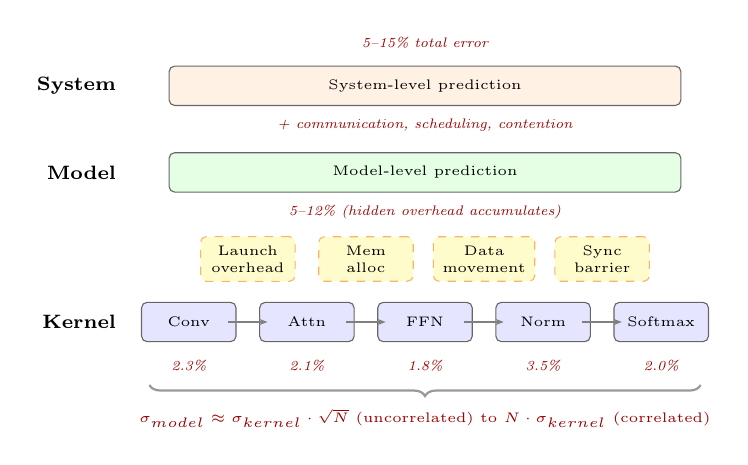
\begin{tikzpicture}[
    box/.style={draw=black!60, rounded corners=2pt, minimum width=1.2cm, minimum height=0.5cm, align=center, font=\tiny},
    err/.style={font=\tiny\itshape, text=red!60!black},
    arr/.style={-{Stealth[length=3pt]}, thick, black!50},
    brace/.style={decorate, decoration={brace, amplitude=4pt, mirror}, thick, black!40},
]

% Kernel level
\node[box, fill=blue!10] (k1) at (0,0) {Conv};
\node[box, fill=blue!10] (k2) at (1.5,0) {Attn};
\node[box, fill=blue!10] (k3) at (3,0) {FFN};
\node[box, fill=blue!10] (k4) at (4.5,0) {Norm};
\node[box, fill=blue!10] (k5) at (6,0) {Softmax};
\node[err] at (0,-0.55) {2.3\%};
\node[err] at (1.5,-0.55) {2.1\%};
\node[err] at (3,-0.55) {1.8\%};
\node[err] at (4.5,-0.55) {3.5\%};
\node[err] at (6,-0.55) {2.0\%};
\node[font=\scriptsize\bfseries, anchor=east] at (-0.8,0) {Kernel};

% Composition arrows
\draw[arr] (0.5,0) -- (1,0);
\draw[arr] (2,0) -- (2.5,0);
\draw[arr] (3.5,0) -- (4,0);
\draw[arr] (5,0) -- (5.5,0);

% Hidden errors
\node[box, fill=yellow!20, dashed, draw=orange!60] (h1) at (0.75,0.8) {Launch\\overhead};
\node[box, fill=yellow!20, dashed, draw=orange!60] (h2) at (2.25,0.8) {Mem\\alloc};
\node[box, fill=yellow!20, dashed, draw=orange!60] (h3) at (3.75,0.8) {Data\\movement};
\node[box, fill=yellow!20, dashed, draw=orange!60] (h4) at (5.25,0.8) {Sync\\barrier};

% Model level
\node[box, fill=green!10, minimum width=6.5cm] (model) at (3,1.9) {Model-level prediction};
\node[err] at (3,1.4) {5--12\% (hidden overhead accumulates)};
\node[font=\scriptsize\bfseries, anchor=east] at (-0.8,1.9) {Model};

% System level
\node[box, fill=orange!10, minimum width=6.5cm] (system) at (3,3.0) {System-level prediction};
\node[err] at (3,2.5) {+ communication, scheduling, contention};
\node[font=\scriptsize\bfseries, anchor=east] at (-0.8,3.0) {System};
\node[err] at (3,3.55) {5--15\% total error};

% Braces
\draw[brace] (-0.5,-0.8) -- (6.5,-0.8) node[midway, below=5pt, font=\tiny, text=red!60!black] {$\sigma_{\text{model}} \approx \sigma_{\text{kernel}} \cdot \sqrt{N}$ (uncorrelated) to $N \cdot \sigma_{\text{kernel}}$ (correlated)};

\end{tikzpicture}%
}
\caption{Error composition across abstraction levels. Kernel-level predictions (2--3\% each) accumulate through hidden overheads (kernel launch, memory allocation, data movement, synchronization) that are not captured by kernel-level tools, yielding 5--12\% model-level error. System-level errors add communication and scheduling overhead.}
\label{fig:error-composition}
\end{figure}

\textbf{Emerging hardware and future directions.}
PIM~\cite{upimulator2024,attacc2024,neupims2024,paise2025}, chiplets, and disaggregated designs blur memory hierarchy assumptions; FlashAttention~\cite{flashattention2022} changes the landscape faster than models retrain; no MLPerf~\cite{mlperf_training2020,mlperf_inference2020} equivalent exists for performance \emph{prediction}.
Key future directions: (1)~a common evaluation benchmark for modeling tools; (2)~validated tools for frontier workloads; (3)~formal composition error bounds; (4)~unified energy-latency-memory prediction~\cite{mlperfpower2025}; (5)~Docker-first deployment with portable formats (ONNX, Chakra~\cite{chakra2023}).

% ==============================================================================
% CONCLUSION
% ==============================================================================
\section{Conclusion}
\label{sec:conclusion}

This survey analyzed 22 tools in depth for predicting ML workload performance, organized by methodology type, target platform, and abstraction level.
Key findings:
(1)~\emph{No single methodology dominates}---analytical models offer microsecond interpretable evaluation, trace-driven simulators provide 2--15\% system-level error, and hybrid approaches achieve the best accuracy--speed balance (NeuSight: 2.3\% MAPE), with the right choice depending on the practitioner's priorities.
(2)~\emph{LLM workloads demand specialized modeling}---prefill/decode distinctions, KV cache management, and dynamic batching require purpose-built tools (VIDUR, Frontier) rather than CNN-era extensions.
(3)~\emph{Reproducibility is a practical bottleneck}---Docker-first tools remain reproducible while tools relying on serialized ML models have become unusable.
(4)~\emph{Accuracy claims require scrutiny} due to varying benchmarks and metrics.

The most pressing gaps are closing the temporal validation lag for frontier workloads (MoE, diffusion, dynamic inference), establishing common evaluation benchmarks for rigorous cross-tool comparison, solving kernel-to-end-to-end error composition, supporting emerging hardware (PIM, chiplets), and addressing reproducibility failures.
As ML workloads grow in scale and diversity, this survey provides practitioners guidance for tool selection and researchers a roadmap for advancing the field.

%%%%%%% -- PAPER CONTENT ENDS -- %%%%%%%%

%%
%% The next two lines define the bibliography style to be used, and
%% the bibliography file.
\bibliographystyle{ACM-Reference-Format}
\bibliography{references}

\end{document}
